\documentclass{article}
\usepackage{spconf,amsmath,amssymb,graphicx,booktabs,multirow,placeins,array}
\usepackage[table]{xcolor}
\usepackage{flafter,balance,capt-of,float,tabularx}
\usepackage{hyperref}
\DeclareMathSizes{8}{8}{6}{5}
\definecolor{valfill}{RGB}{231,239,249}
\definecolor{testfill}{RGB}{224,239,234}
\definecolor{basefill}{RGB}{248,249,251}
\definecolor{conffill}{RGB}{255,247,231}
\definecolor{learnfill}{RGB}{235,246,240}
\definecolor{valink}{RGB}{38,83,123}
\definecolor{testink}{RGB}{34,93,82}
\definecolor{confink}{RGB}{142,91,24}
\definecolor{learnink}{RGB}{30,99,78}
\definecolor{upgreen}{RGB}{24,115,62}
\definecolor{downred}{RGB}{169,48,46}
\definecolor{samegray}{RGB}{95,102,112}
\newcommand{\upchg}[1]{\,\textcolor{upgreen}{(\ensuremath{\uparrow#1})}}
\newcommand{\downchg}[1]{\,\textcolor{downred}{(\ensuremath{\downarrow#1})}}
\newcommand{\callup}[1]{\,\textcolor{downred}{(\ensuremath{\uparrow#1})}}
\newcommand{\calldown}[1]{\,\textcolor{upgreen}{(\ensuremath{\downarrow#1})}}
\newcommand{\samechg}[1]{\,\textcolor{samegray}{(=#1)}}

\hypersetup{hidelinks,pdftitle={When Should a Vision Specialist Defer? Budgeted Collaboration with Vision-Language Models},pdfauthor={Sihang Cai, Rongjunchen Zhang, Tao Jin}}
\title{When Should a Vision Specialist Defer?\\Budgeted Collaboration with Vision--Language Models}
\name{Sihang Cai$^1$ \qquad Rongjunchen Zhang$^1$ \qquad Tao Jin$^2$}
\address{$^1$HiThink Research \qquad $^2$Zhejiang University}
\setlength{\emergencystretch}{1em}
\raggedbottom
\renewcommand{\dbltopfraction}{0.90}
\renewcommand{\textfraction}{0.10}
\setcounter{dbltopnumber}{2}
\setlength{\dbltextfloatsep}{10pt plus 2pt minus 2pt}
\setlength{\textfloatsep}{9pt plus 2pt minus 2pt}
\begin{document}
\ninept
\maketitle
\begin{abstract}
When should a vision specialist call a general vision--language model (VLM)? A specialist's low confidence does not tell us whether the VLM will give a better answer. We study this decision across 4 visual tasks and 16 model pairs. Our Learned Routing (LR) method uses the input and the specialist's outputs to estimate whether replacing its answer will help or hurt. A normalized score ranks inputs for VLM calls, with its normalization strength and threshold chosen on validation data. We evaluate performance over the full 0--100\% call range. At validation-selected thresholds, LR exceeds both standalone models in 10 pairs, using means over five training seeds. We also compare different training objectives and ways of constructing the ranking score. In some tasks, changing the score without retraining has a larger effect than changing among the tested objectives. The best score varies across tasks, and some model pairs benefit little from collaboration. Code: \url{https://github.com/nohi191212/ModelCollaboration}.

\end{abstract}
\begin{keywords}
Model collaboration, visual recognition, learning to defer, budgeted inference
\end{keywords}
\section{Introduction}
Task-specific vision models offer efficient predictions, while general vision--language models (VLMs) can handle a broader range of inputs at greater computational cost. Calling a VLM only when needed may improve accuracy without paying this cost on every input, a motivation also reflected in prompt-routing services~\cite{bedrockrouting}. We consider a system in which a specialist first predicts a class, a set of boxes or an event label. A router then decides whether to keep that answer or replace it with the VLM's answer.

A natural rule is to call the VLM when the specialist has low confidence. However, uncertainty alone does not show whether the replacement will help. The VLM may fail on the same example, or overturn an answer that was already correct. Even a VLM with lower average accuracy can be useful if its strengths complement those of the specialist. Routing must therefore learn where the two models differ, rather than only where the specialist is uncertain.

Prior work offers several starting points. Confidence estimation~\cite{calibration} and selective prediction~\cite{selectivenet} identify uncertain inputs. Learning to defer also accounts for an imperfect expert~\cite{defer,calibrateddefer}. Its joint-classification formulations learn class outputs alongside deferral, changing the retained predictor and requiring adaptation for box or event outputs. Post-hoc deferral~\cite{posthocdefer} keeps an existing predictor fixed, making it a closer comparison for answer replacement. We adapt its loss to our router inputs and backbone. Text routing and cascading~\cite{frugal,routellm,cascaderouting} and multimodal routing~\cite{vlrouterbench,mmrbench,relope,streamsense} address related choices, but their model interfaces and evaluation settings require adaptation here. Speculative decoding~\cite{specdecode,specsampling} verifies draft tokens rather than choosing between completed visual answers.

We introduce \textbf{Learned Routing (LR)}, a compact router that uses input features, specialist representations, predictions and confidence. During training, answers from both models reveal when replacement helps or hurts. At inference, LR uses only information available before the VLM call. We distinguish what the router learns from how its outputs rank inputs: the same trained model can produce different rankings when its score is changed. Our default normalizes estimated replacement gains, choosing the normalization strength on validation data.

Our contributions are as follows.

\noindent\textbf{(1) Unified evaluation.} We bring confidence routing, LR and post-hoc deferral~\cite{posthocdefer} into cross-task experiments spanning fine-grained recognition, grounding, two-image reasoning and safety-event recognition. Across 16 model pairs, full-call-range curves show where collaboration improves performance and where the specialist alone is preferable.

\noindent\textbf{(2) Routing method and empirical finding.} We develop a compact router with a normalized ranking score, and compare training objectives separately from score construction. In some tasks, changing the score without retraining has a larger effect than changing among the tested objectives. The preferred score remains task-dependent.

\noindent\textbf{(3) Open-source release.} We release all experiment code and per-example experimental data, the 80 router checkpoints used in the main table, and the configurations, prompts and reproduction scripts. These materials support retraining the routers, reconstructing the reported curves and comparing additional methods.

\section{Preliminary}
\label{sec:preliminary}

Let $S$ be a specialist and $L$ a VLM. For input $x$, the specialist first gives $S(x)$. A router then uses information $\mathcal I(x)$ available before calling $L$ to choose the final answer:
\begin{equation}
\widehat y(x)=
\begin{cases}S(x),&a(x)=0,\\L(x),&a(x)=1,\end{cases}
\quad a(x)\in\{0,1\}.
\label{eq:decision}
\end{equation}
Here $a(x)=0$ keeps the specialist answer, while $a(x)=1$ calls the VLM and uses its answer instead.

For $n$ inputs, $\sum_i a(x_i)$ is the number of VLM calls. Given an allowed call fraction $b$, we seek the highest task score $M$:
\begin{equation}
\max_a M(\widehat{\mathbf y},\mathbf y)
\quad\text{s.t.}\quad \sum_i a(x_i)\leq\lfloor bn\rfloor.
\label{eq:budget}
\end{equation}
Here $\widehat{\mathbf y}$ and $\mathbf y$ collect the final answers and ground-truth labels. For example, $b=0.25$ allows calls on at most a quarter of the inputs. Each input counts once, even if it contains two images or multiple target objects. Our router makes this choice using a score threshold chosen on validation data. The same threshold is used on test inputs, where the fraction of calls may differ from the validation budget.


% Page 2: method illustration, distillation and routing, then selection criterion.
\twocolumn[{
\begin{minipage}{\textwidth}
\centering
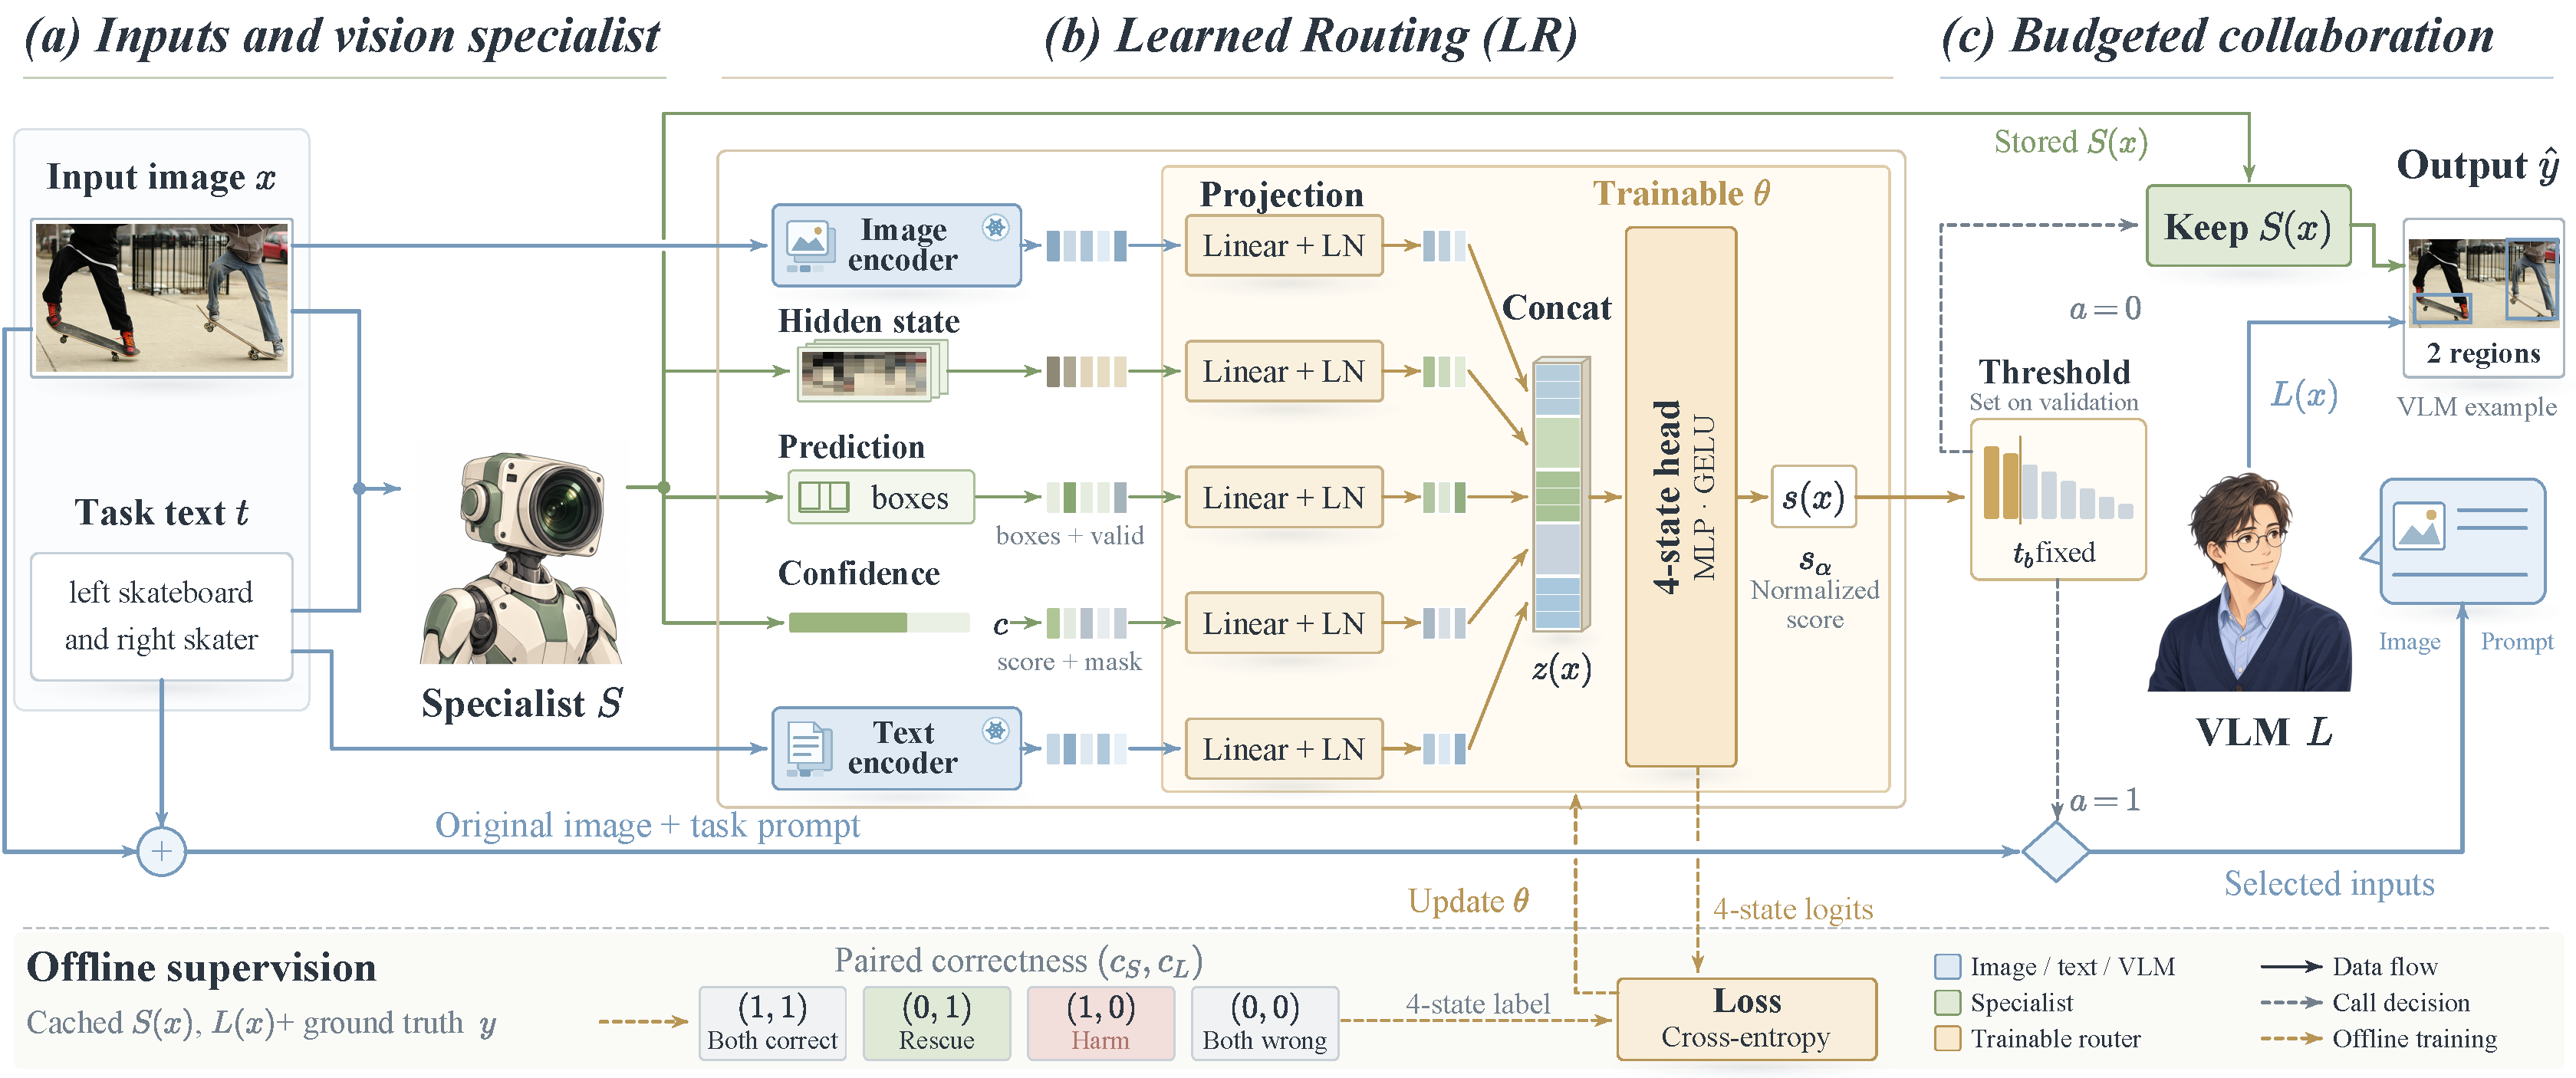
\includegraphics[width=\textwidth]{figures/method.pdf}
\captionof{figure}{\textbf{Deciding when to call the VLM.} After the specialist predicts, LR combines input and specialist features. The illustrated four-state variant estimates paired outcomes and normalizes its score before a validation-selected threshold decides whether to retain the specialist answer or call the VLM. Image-only tasks omit text.}
\label{fig:method}
\end{minipage}\vspace{10pt}
}]
\nobalance
\section{Learned Routing}
\label{sec:method}
\subsection{Replacement Outcomes and Gain}
Let $c_S,c_L\in\{0,1\}$ indicate specialist and VLM correctness. Their paired outcomes are both correct $(1,1)$, rescue $R=(0,1)$, harm $H=(1,0)$ and both wrong $B=(0,0)$. For delegated inputs $A$,
\begin{equation}
\Delta\operatorname{Acc}=\frac{|R\cap A|-|H\cap A|}{n}.
\label{eq:decomposition}
\end{equation}
Given pre-call information $\mathcal I$, expected correctness gain is
\begin{equation}
\eta(\mathcal I)=\Pr(R\mid\mathcal I)-\Pr(H\mid\mathcal I).
\label{eq:utility}
\end{equation}
With true conditional probabilities and equal call costs, choosing the largest positive gains maximizes expected accuracy under a budget ceiling. Network probabilities are estimates; alternative scores can rank them differently. Macro-F1 is not additive, so construction performance is computed from the combined predictions rather than this gain identity.

\subsection{Shared Inputs and Supervision}
LR uses an 8.07M-parameter image/text backbone distilled from SigLIP2~\cite{siglip2} on training inputs. Distillation matches normalized image and text features separately, without task labels. The backbone and specialist remain frozen during router training.

Figure~\ref{fig:method} combines image features, pooled specialist states, prediction summaries and confidence with missing-value indicators. Task text adds a branch on gRefCOCO and NLVR2. Each branch is projected to 128 dimensions and layer-normalized; their concatenation enters an MLP with 128 hidden units and GELU. Each pair learns separate weights under shared settings.

Our four-state version, $\mathrm{LR}_{4S}$, uses one target state per example, or fractions over four construction events. We minimize
\begin{equation}
\mathcal L_{4S}=-\frac1N\sum_{i=1}^{N}\sum_{k=1}^{4}q_{ik}\log p_{ik},
\qquad p_i=\operatorname{softmax}(\ell_i).
\label{eq:loss}
\end{equation}
Here $q_i$ is the observed state distribution. Four outputs support outcome inspection and several scoring rules; we do not assume that distinguishing both-correct from both-wrong cases must improve ranking. We use uniform sampling without class weights or label smoothing.

For the post-hoc comparison $\mathrm{LR}_{PH}$, a scalar head $r$ on the same inputs uses the deferral loss~\cite{posthocdefer}
\begin{equation}
\mathcal L_{PH}=e_S\log(1+e^{-r})+e_L\log(1+e^{r}),
\label{eq:posthoc}
\end{equation}
where $e_S=1-c_S$ and $e_L=1-c_L$ (event averages for construction). We fix the added call-cost coefficient to zero and sweep the score threshold to compare budgets. The original specialist answer is retained when no call is made.

\subsection{From Outcome Estimates to a Ranking}
Our default $\mathrm{LR}_{4S}$ uses
\begin{equation}
s_\alpha(x)=\frac{p_R-p_H}{(p_R+p_H+2p_B+\epsilon)^\alpha},
\quad \epsilon=10^{-8}.
\label{eq:score}
\end{equation}
At $\alpha=0$ this is the probability difference. Ignoring $\epsilon$, $\alpha=1$ ranks like the estimated error-rate ratio $(p_R+p_B)/(p_H+p_B)$. Intermediate values interpolate between these rankings. Normalization uses existing outputs, not new information or a VLM call. It is an empirical scoring rule and does not inherit the true-gain optimality statement above.

\subsection{Full-Budget Selection}
\label{sec:selection}
For a score, let $M(u_k)$ be validation performance after delegating its top $\lfloor kn/100\rfloor$ inputs, with $u_k=\lfloor kn/100\rfloor/n$. We evaluate the full curve,
\begin{equation}
\mathcal A_{100}=\sum_{k=1}^{100}\frac{M(u_{k-1})+M(u_k)}2(u_k-u_{k-1}).
\label{eq:area}
\end{equation}


% Page 3: main table, threshold selection and dataset table left, implementation/results right.
\clearpage
\nobalance
\twocolumn[{\begin{minipage}{\textwidth}
\centering
\captionof{table}{Test results at validation-selected thresholds over 0--100\% budgets. Scores and actual calls are percentages; LR is normalized $\mathrm{LR}_{4S}$, averaged over five seeds. Parentheses show LR-minus-confidence changes in percentage points (green: better; red: worse). Bold marks the higher routed score; $\dagger$ exceeds both endpoints. M: MiniCPM-V-4.5; Q: Qwen3.8-27B-FP8.}
\label{tab:main}
\fontsize{9}{10.8}\selectfont
\setlength{\tabcolsep}{3.0pt}
\renewcommand{\arraystretch}{1.03}
\begin{tabular}{@{}lllrr>{\columncolor{conffill}}r>{\columncolor{conffill}}r>{\columncolor{learnfill}}r>{\columncolor{learnfill}[\tabcolsep][0pt]}r@{}}
\toprule
\multirow{2}{*}{Dataset} & \multirow{2}{*}{Specialist} & \multirow{2}{*}{VLM} & \multicolumn{2}{c}{Standalone} & \multicolumn{2}{c}{Confidence} & \multicolumn{2}{c}{LR} \\
\cmidrule(lr){4-5}\cmidrule(lr){6-7}\cmidrule(l){8-9}
 & & & Spec. & VLM & Score$\uparrow$ & Calls$\downarrow$ & Score$\uparrow$ & Calls$\downarrow$ \\
\midrule
CUB-200-2011 & ResNet & M & 81.43 & 26.56 & \textbf{81.43} & 0.00 & \textbf{81.43}\samechg{0.00} & 0.59\callup{0.59} \\
 & ResNet & Q & 81.43 & 54.82 & \textbf{81.43} & 0.00 & \textbf{81.43}\samechg{0.00} & 0.00\samechg{0.00} \\
 & GLSim & M & 90.16 & 26.56 & \textbf{90.16} & 0.00 & 90.13\downchg{0.03} & 0.85\callup{0.85} \\
 & GLSim & Q & 90.16 & 54.82 & \textbf{90.16} & 0.00 & \textbf{90.16}\samechg{0.00} & 0.00\samechg{0.00} \\
\midrule
gRefCOCO & GroundingDINO & M & 26.69 & 50.01 & 50.01 & 100.00 & \textbf{50.23}$^\dagger$\upchg{0.22} & 58.19\calldown{41.81} \\
 & GroundingDINO & Q & 26.69 & 74.47 & 74.47 & 100.00 & \textbf{75.12}$^\dagger$\upchg{0.65} & 88.47\calldown{11.53} \\
 & InstanceVG & M & 66.95 & 50.01 & 61.88 & 52.09 & \textbf{67.91}$^\dagger$\upchg{6.04} & 19.04\calldown{33.06} \\
 & InstanceVG & Q & 66.95 & 74.47 & 72.43 & 68.39 & \textbf{76.24}$^\dagger$\upchg{3.81} & 62.00\calldown{6.38} \\
\midrule
NLVR2 & BEiT3 & M & 80.00 & 90.74 & 90.77 & 85.80 & \textbf{90.80}$^\dagger$\upchg{0.03} & 91.10\callup{5.30} \\
 & BEiT3 & Q & 80.00 & 90.06 & 90.24 & 85.80 & \textbf{90.60}$^\dagger$\upchg{0.36} & 84.34\calldown{1.46} \\
 & ViLT & M & 76.42 & 90.74 & 90.64 & 95.93 & \textbf{90.69}\upchg{0.05} & 98.06\callup{2.13} \\
 & ViLT & Q & 76.42 & 90.06 & 89.96 & 95.93 & \textbf{90.07}$^\dagger$\upchg{0.10} & 99.62\callup{3.69} \\
\midrule
ConstructionSite & YOLO26x & M & 18.13 & 22.36 & 25.23 & 92.54 & \textbf{25.88}$^\dagger$\upchg{0.65} & 45.32\calldown{47.22} \\
 & YOLO26x & Q & 18.13 & 27.00 & 25.97 & 92.21 & \textbf{29.80}$^\dagger$\upchg{3.82} & 44.77\calldown{47.44} \\
 & RT-DETR-X & M & 7.89 & 22.36 & 22.36 & 100.00 & \textbf{22.80}$^\dagger$\upchg{0.44} & 78.44\calldown{21.56} \\
 & RT-DETR-X & Q & 7.89 & 27.00 & \textbf{27.00} & 100.00 & 26.78\downchg{0.22} & 83.57\calldown{16.43} \\
\bottomrule
\end{tabular}
\end{minipage}
\vspace{10pt}}]
Each epoch evaluates $\alpha\in\{0,0.25,0.5,0.75,1\}$. Validation $\mathcal A_{100}$ jointly selects the checkpoint and $\alpha$; ties favor smaller $\alpha$ within an epoch and earlier epochs across training. Early stopping uses the same criterion. Cross-entropy itself is unchanged. Table~\ref{tab:main} abbreviates normalized $\mathrm{LR}_{4S}$ as LR.

To select a threshold, validation budgets range from 0 to 100\% in 1\% steps. At each interior budget, a cutoff includes tied scores only if all fit the quota. The highest validation task score selects the threshold; ties favor fewer calls and then a smaller budget. Endpoints mean never or always calling the VLM.

The cutoff and comparison operator transfer unchanged to test inputs; actual test calls can differ from the nominal validation budget. Confidence uses the same threshold search with negative maximum class probability or detection confidence, prioritizing missing confidence. Test labels select neither scores nor thresholds.

{\setlength{\intextsep}{3pt}\section{Experiments}
\subsection{Datasets and Metrics}
\label{sec:implementation}
\begin{table}[H]
\centering
\caption{Datasets, tasks and dataset split sizes.}
\label{tab:data}
\fontsize{9}{10.8}\selectfont
\setlength{\tabcolsep}{1.2pt}
\begin{tabularx}{\columnwidth}{@{}l>{\raggedright\arraybackslash}Xrrr@{}}
\toprule
\rowcolor{valfill} Dataset & Task & Train & Val. & Test\\
\midrule
CUB-200-2011 & Fine-grained classification & 4,792 & 1,200 & 5,794\\
gRefCOCO & Semantic grounding & 209,344 & 14,229 & 35,263\\
NLVR2 & Visual reasoning & 85,042 & 6,982 & 13,937\\
ConstructionSite & Event detection & 6,308 & 701 & 3,004\\
\bottomrule
\end{tabularx}
\end{table}

}
CUB~\cite{cub} evaluates bird recognition and NLVR2~\cite{nlvr2} evaluates two-image reasoning. Both use accuracy. Table~\ref{tab:data} counts images for CUB and ConstructionSite, expressions for gRefCOCO, and paired-image statements for NLVR2.

gRefCOCO~\cite{gref} evaluates whole-expression box correctness. After filtering boxes with scores below 0.7, greedy matching at generalized IoU $\geq 0.5$ must leave no missed or extra instances. No-target expressions require valid empty outputs. This differs from official segmentation evaluation.

ConstructionSite~\cite{construction} uses macro-F1 across personal-protection, fall-protection, unprotected-edge and excavator-proximity violations, with one routing decision per image.

{\setlength{\intextsep}{3pt}\subsection{Implementation and Comparisons}
Specialists are ResNet-50~\cite{resnet}, GLSim~\cite{glsim}, GroundingDINO~\cite{groundingdino}, InstanceVG~\cite{instancevg}, BEiT3~\cite{beit3}, ViLT~\cite{vilt}, YOLO26X~\cite{yolo26} and RT-DETR-X~\cite{rtdetr}. Each pairs with MiniCPM-V-4.5~\cite{minicpm} (M) and Qwen3.8-27B-FP8~\cite{qwen38} (Q).

LR uses AdamW, learning rate 0.003, weight decay 0.01, batch 256, at most 50 epochs and patience 8. Specialist states are taken at 90\% depth. We retain the architecture from an earlier eighteen-setting search and repeat training with seeds 2026--2030. Main results use the full-budget selection above; Table~\ref{tab:objective} uses earlier training settings, detailed in the supplement.

Each VLM receives one temperature-zero request per example. Invalid responses remain errors and are never repaired. The supplement reports per-seed results, full curves and additional training comparisons. These analyses reuse previously inspected test sets and are exploratory, rather than a new blind evaluation.
}
\subsection{Main Results Analysis}
Table~\ref{tab:main} shows pair-dependent benefits: useful delegation recovers specialist errors while avoiding harmful replacements.

For bird recognition, the tested VLMs rarely justify replacing the specialist; retaining its answer is the practical default. Grounding offers clearer complementarity, especially with InstanceVG. Visual reasoning favors extensive VLM use, limiting call savings. Construction benefits vary: YOLO gains from selective delegation, whereas RT-DETR-X/Q does not improve on its VLM endpoint. The comparison should therefore include both standalone models and assess the full curve; collaboration need not beat either standalone model.


% Page 4: gain figure, analysis/comparisons left, costs/conclusion right.
\twocolumn[{
\begin{minipage}{\textwidth}
\centering
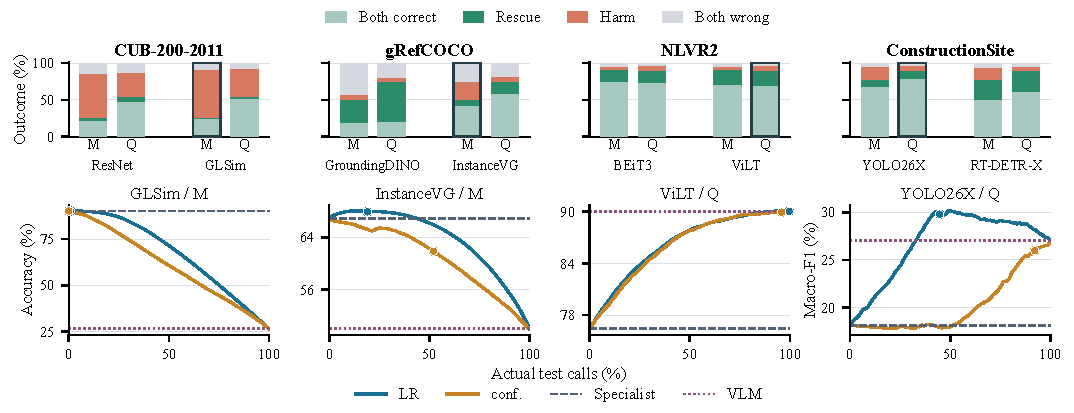
\includegraphics[width=0.96\textwidth]{figures/gains_compact.pdf}
\captionof{figure}{\textbf{Collaboration gains on test data.} Top: paired outcomes for all 16 pairs; outlines identify the pairs below. Construction counts events, other tasks examples. Bottom: performance versus actual calls, including both endpoints. LR lines average five seeds; dots show mean results at independently selected validation thresholds.}
\label{fig:gains}
\end{minipage}\vspace{10pt}
}]
\subsection{Where Collaboration Gains Come From}
\label{sec:gains}
Figure~\ref{fig:gains} relates paired outcomes to test-call curves. With the selected thresholds, InstanceVG/M corrects 727.6 expressions but introduces 388.2 errors on average, adding 0.96 accuracy points. GLSim/M has only 106 rescuable images against 3,791 harmful replacements, favoring few calls. Construction has 96.37\% negative event labels. Correct negatives contribute to outcome shares but not macro-F1.

We also compare at identical actual calls. After normalization, full-budget checkpoint reselection changes task-average curves by just $+0.065$, $+0.068$, $+0.102$ and $-0.010$ points, respectively. The larger scoring effects below are therefore not explained solely by low-budget checkpoint selection.

{\setlength{\intextsep}{1pt}\subsection{Supervision, Scoring and Post-hoc Deferral}
\label{sec:ablation}
\noindent\begin{minipage}{\columnwidth}
\centering
\captionof{table}{Full-budget means (\%). Avg.: equal-task mean (five-seed SD). $\Delta$: gain over $\mathrm{LR}_{PH}$ (pp). Shared weights for $\mathrm{LR}_{4S}$. Earlier selection settings in supplement. CS: ConstructionSite.}
\label{tab:objective}
\fontsize{8}{9.5}\selectfont
\setlength{\tabcolsep}{1.5pt}
\begin{tabular}{@{}llrrrrrr@{}}
\toprule
Variant & Score & CUB & gRef & NLVR & CS & Avg. & $\Delta$ \\
\midrule
$\mathrm{LR}_{PH}$ & $r$ & 65.86 & 59.37 & 87.33 & 21.24 & 58.45 (0.07) & -- \\
\midrule
3-state & $p_R-p_H$ & 71.27 & 60.13 & 86.34 & 21.77 & 59.88 (0.06) & \textcolor{upgreen}{+1.43} \\
Gain & $\widehat\Delta$ & 71.01 & 59.97 & 86.29 & 21.61 & 59.72 (0.04) & \textcolor{upgreen}{+1.27} \\
\midrule
$\mathrm{LR}_{4S}$ & $p_R-p_H$ & 71.30 & 60.10 & 86.43 & 21.69 & 59.88 (0.06) & \textcolor{upgreen}{+1.43} \\
$\mathrm{LR}_{4S}$ & $\log(p_R/p_H)$ & 67.80 & 59.84 & 87.36 & 21.11 & 59.03 (0.09) & \textcolor{upgreen}{+0.58} \\
$\mathrm{LR}_{4S}$ & $r_{4S}$ & 67.63 & 59.90 & 87.36 & 21.30 & 59.05 (0.10) & \textcolor{upgreen}{+0.60} \\
\rowcolor{learnfill}
$\mathrm{LR}_{4S}$ & $s_\alpha$ & 71.37 & 60.66 & 87.36 & 21.63 & 60.25 (0.06) & \textcolor{upgreen}{+1.81} \\
\bottomrule
\end{tabular}

\end{minipage}\par\vspace{4pt}
Table~\ref{tab:objective} compares training objectives and scores. Merging the two unchanged outcomes into one target or directly predicting the gain gives curves close to the four-state probability difference. The supplement gives their losses and training settings.

Changing only the score has a larger effect on some tasks. Here $r_{4S}=\log[(p_R+p_B)/(p_H+p_B)]$ estimates the optimal score of the post-hoc loss~\cite{posthocdefer}, whereas $\mathrm{LR}_{PH}$ learns its score directly. On NLVR2, this change largely closes the middle-to-high-budget gap to post-hoc deferral, but it hurts CUB. The normalized score has the highest task average, while no score is best on every task.
}
\subsection{Computational Cost}
\label{sec:cost_provisional}
\noindent\begin{minipage}{\columnwidth}
\centering

\includegraphics[width=0.86\columnwidth]{figures/cost_compact.pdf}
\captionof{figure}{\textbf{Cost--performance trade-offs.} InstanceVG/M (left), YOLO26X/Q (right). LR curves show five-seed means with one-SD bands. Dots average results at validation-selected thresholds. Costs are component-based estimates.}
\label{fig:cost}
\end{minipage}\par\vspace{4pt}
We add specialist and router costs per input, plus VLM cost at the actual call rate. Confidence omits router overhead. Existing A800 component measurements provide serial cost estimates, not newly measured integrated latency.

InstanceVG/M gains 6.04 points over confidence with 63.3\% fewer estimated FLOPs and 61.3\% less time; YOLO26X/Q gains 3.82 points with reductions of 51.4\% and 50.9\%.

\section{Conclusion}
Learned Routing separates estimating replacement outcomes from ranking inputs for delegation. In some tested regimes, scoring affects performance more than the choice among gain-related targets. Validation-selected normalization offers a practical compromise, and allowing zero calls avoids unnecessary replacements. Benefits remain pair-dependent: neither four-state supervision nor a fixed ratio is universally superior.

\clearpage
\balance
\begin{center}\bfseries COMPLIANCE WITH ETHICAL STANDARDS\end{center}
\noindent This study did not require ethical approval. The authors declare no actual or potential conflicts of interest.
\bibliographystyle{IEEEbib}
\bibliography{references}
\end{document}
